\documentclass[a4paper, 12pt]{article} %type 

% Russian Language
\title{Отчет по лабораторной работе №2 по теме: "Задача о распаде разрыва для системы уравнений акустики"}
\author{Латарцев Павел Б05-902б группа}
\date{2023}

\usepackage[left=1cm, top=2cm, right=1cm, bottom=2cm, nohead, nofoot]{geometry}
\usepackage[warn]{mathtext}
\usepackage[T2A]{fontenc}
\usepackage[utf8]{inputenc}
\usepackage[english, russian]{babel}
\usepackage{tikz}
\usepackage{lipsum}

\usepackage{amsmath,amssymb}
\usepackage{amsthm}

\usepackage{verbatim}

%\usepackage[demo]{graphicx}
\usepackage{caption}

\usepackage{hyperref}

\newcommand{\p}[1]{\mathbb{P}(#1)}
\newcommand{\E}{\mathbb{E}}
\newcommand{\D}{\mathbb{D}}

\begin{document}

\maketitle

\section{Условие} 

\subsection{Задача}

\begin{equation*}
 \begin{cases}
	\frac{\partial u}{\partial t} + \frac{1}{\rho_{0}}\frac{\partial p}{\partial x} = 0 \\
	\frac{\partial p}{\partial t} + \rho_{0} c_{0} \frac{\partial p}{\partial x} = 0
 \end{cases}
\end{equation*}

\begin{equation*}
u(0, x) =  
 \begin{cases}
	u_L, \,\,\, x < 0 \\
	u_R, \,\,\, x > 0
 \end{cases} 
\end{equation*}

\begin{equation*}
p(0, x) =  
 \begin{cases}
	p_L, \,\,\, x < 0 \\
	p_R, \,\,\, x > 0
 \end{cases}
\end{equation*}

\subsection{Шаблон}

Шаблон № 6, начальное условие «полуэллипс», $\sigma = 0.25$

\begin{figure}[h!]
    \centering
    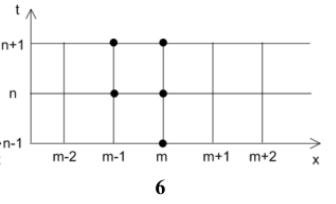
\includegraphics[width=10cm]{shablon.png}
    \caption{Схема шаблона}
    \label{fig:vac}
\end{figure} 

Начальное условие «полуэллипс»:
\begin{equation*}
\varphi(x) = 
 \begin{cases}
   \sqrt{1 - 100 \cdot \left( x - 0.5 \right)^2} &\text{при $0.4 \leqslant x \leqslant 0.6$}\\
   0 &\text{иначе}
\end{cases}
\end{equation*}


\section{Теоритическая часть}
$$\alpha^{0}_{-1} - \text{ось x}, \,\,\,\, \alpha^{0}_{0} - \text{ось y}$$

\subsection{Система}
\begin{equation*}
\varphi(x) = 
 \begin{cases}
 	\alpha^{1}_{-1}\left(1 + \sigma \right) + \alpha^{0}_{-1} - \alpha^{-1}_{0} \sigma = \sigma  \\  
 	\alpha^{1}_{-1} + \alpha^{0}_{-1} + \alpha^{0}_{0} + \alpha^{-1}_{0}  = 1 \\
 	\alpha^{1}_{-1} \left( 1 + 2\sigma + \sigma^2 \right) + \alpha^{0}_{-1} + \alpha^{-1}_{0}\sigma^2 = \sigma^2 \\
 	\alpha^{1}_{-1} \left( 1 + 3\sigma + 3\sigma^2 + \sigma^3 \right) - \alpha^{0}_{-1} + \alpha^{-1}_{0}\sigma^3 = -\sigma^3 
 \end{cases}
\end{equation*}

\subsection{Область монотонности положительных по Фридрихсу $\alpha^\nu_\mu \geqslant 0$ схем}
\label{subsec:1t}
\begin{equation*}
 \begin{cases}
 	\alpha^{0}_{-1} \geqslant 0  \\  
 	\alpha^{0}_{0} \geqslant 0 \\
 	\alpha^{-1}_{0} = \frac{1}{1+2\sigma} - \frac{\sigma}{1 + 2\sigma}\alpha^{0}_{-1} - \frac{1 + \sigma}{1 + 2\sigma}\alpha^{0}_{0} \geqslant 0 \\
 	\alpha^{1}_{-1} = \frac{2\sigma}{1+2\sigma} - \frac{1 + \sigma}{1 + 2\sigma}\alpha^{0}_{-1} - \frac{\sigma}{1 + 2\sigma}\alpha^{0}_{0} \geqslant 0 
 \end{cases}
\end{equation*}

\subsection{Однопараметрическое множество схем 2-го порядка аппроксимации}
\label{subsec:2t}
$$\alpha^{0}_{-1} = \frac{-\sigma-1}{\sigma+1} \alpha^{0}_{0}+ \frac{2}{\sigma+1}$$

\subsection{Единственная схема 3-го порядка аппроксимации}
\label{subsec:3t}
$$\alpha^{0}_{-1} = \frac{2\sigma}{\sigma + 1},\,\, 
  \alpha^{0}_{0} = \frac{2(\sigma - 1)}{\sigma + 1}, \,\,
  \alpha^{-1}_{0} = \frac{\sigma - 1}{2\sigma^2 + 3\sigma + 1},\,\,
  \alpha^{1}_{-1} = \frac{2\sigma(\sigma-1)}{(\sigma+1)(2\sigma + 1)}$$


%\subsection{Схема 2-го порядка аппроксимации наиболее близкая к множеству положительных по Фридрихсу схем}

\subsection{Аналитический вид схемы с минимальной «аппроксимационной вязкостью»}
\label{subsec:4t}
$$\alpha^{0}_{-1} = \sigma, \,\,\, \alpha^{0}_{0} = 1-\sigma$$

\subsection{Наиболее близкая ко множеству положительных по Фридрихсу схем среди схем 2-го порядка аппроксимации}
\label{subsec:5t}
$$\alpha^{0}_{-1} = 0.55, \,\,\, \alpha^{0}_{0} = 1.05$$

\subsection{Рисунок для заданного шаблона и числа Куранта}
\label{subsec:6t}
\begin{figure}[h!]
    \centering
    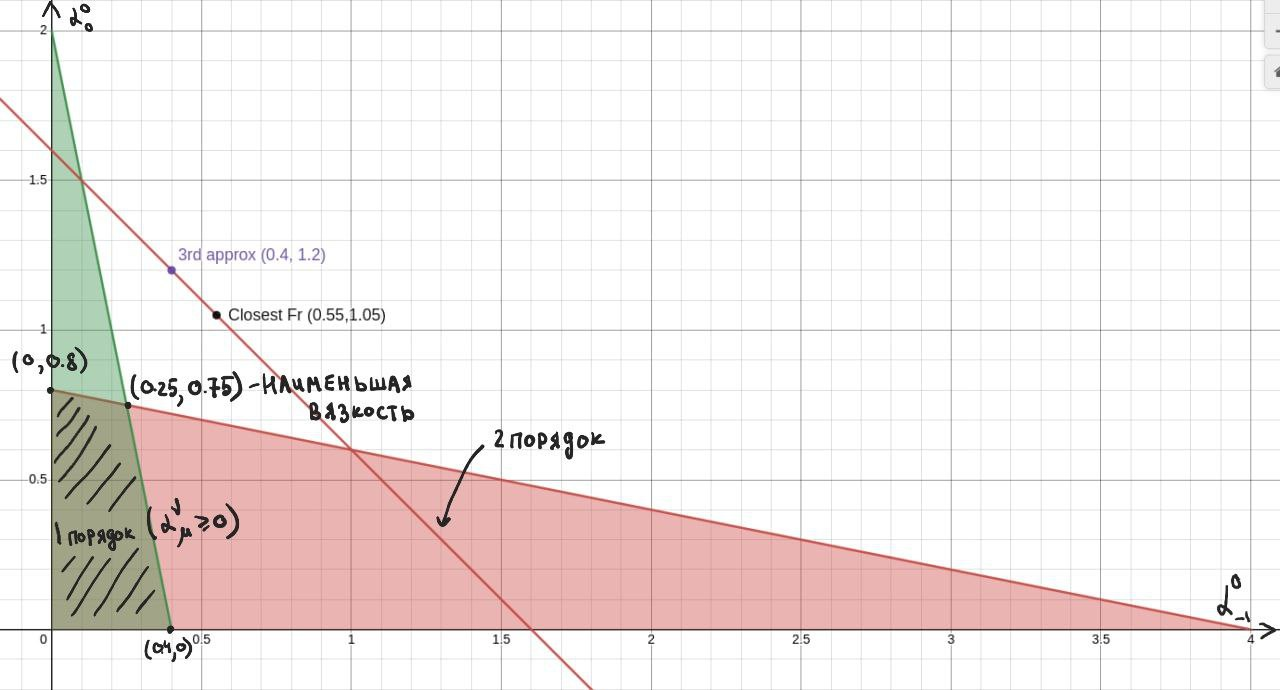
\includegraphics[width=17cm]{risunok.jpg}
    \caption{Рисунок для заданного шаблона и числа Куранта $\sigma = 0.25$}
    \label{fig:vac}
\end{figure} 


\section{Практическая часть}








\end{document}


\begin{figure}[h!]
    \centering
    \includegraphics[width=10cm]{../graphs/difference_Third_order_approximationSecond_order_approximation_1Second_order_approximation_2First_order_approximation_right_up.png}
    \caption{График разности численного и аналитического решения из \ref{subsec:7p} \\ }
    \label{fig:vac}
\end{figure}



\begin{figure}[h!]
    \centering
    \includegraphics[width=20cm]{pr2.png}
    \caption{Функия распределения $\xi, \eta$.}
    \label{fig:vac}
\end{figure} 
